\chapter{The Hidden Markov model}

This chapter is accompanied by a formulary, which can be found in
Appendix~\ref{sec:appendix-formulary} on page~\pageref{sec:appendix-formulary}.
The definition of the Hidden Markov model, the forward algorithm, backward
algorithm and Baum-Welch algorithm in this chapter are from
\cite[pp.~210]{jm09}, except where otherwise noted.

\begin{definition}
 A \emph{Hidden Markov model} (HMM) is a quintuple\footnote{This definition
 diverges in structure from \cite{jm09} in one significant way: It uses a
 single state $\#$ instead of a pair of initial state $q_0$ and final state
 $q_F$. This allows us to use a single probability distribution $t$ to describe
 all state transitions, instead of the triple of matrices $(a_{0i})_i$,
 $(a_{ij})_{(i,j)}$, and $(a_{iF})_i$ that appear in \cite{jm09}.} $\uh =
 (Q,V,\#,t,e)$ such that
 \begin{itemize}\setlength\itemsep{-0.3em}
  \item $Q$ is a non-empty alphabet (of \emph{states}),
  \item $V$ is a non-empty alphabet (of \emph{words}),
  \item $\#\notin Q\cup V$ is a separate (\emph{initial} and \emph{final}) state,
  \item $t\in\um(Q\cup\brc{\#}\!|Q\cup\brc{\#})$ is a transition probability distribution, and
  \item $e\in\um(V|Q)$ is an emission probability distribution. \qedhere
 \end{itemize}
\end{definition}

From here on, we will abbreviate $Q\cup\brc{\#}$ as $Q_\#$.

The Hidden Markov model describes a sentence as being the result of the
progression of a probabilistic state machine that starts out in $\#$, traverses
states from $Q$, and in the end reaches $\#$ again. Each time a state from $Q$
is reached, a word from $V$ is emitted. The sequence of all these emitted words
is the sentence that is observed.

When a sentence $v = v_1\cdots v_n\isin V^*$ is observed, is must have been
caused by a certain sequence of states $q = q_1\cdots q_n\isin Q^*$, but it is
not known which one it was, only that the lengths of both sequences agree.
Therefore, by the law of total probability,
\[
 P(v) = \sum_{q\in Q^n} P(v,q) = \sum_{q\in Q^n} P(v|q) \cdot P(q).
\]

%TODO find a reference for "Markov property" (this paragraph is currently more
%or less copied from en.wikipedia)
\begin{definition}
 A stochastic process is said to have the \emph{Markov property} if the
 conditional probability distribution of the next state of the process only
 depends on the present state, not on the states before it.
\end{definition}

A Hidden Markov model exhibits the Markov property in two separate ways: First,
the conditional probability distribution of each state depends only on the
state directly preceding it. Second, the conditional probability distribution
of each emitted word depends only on the state that was inhabited at the time
of emission. These two conditional probability distributions are called $t$ and
$e$, and are part of the quintuple $\uh=(Q,V,\#,t,e)$ as defined above.

The progression of the probabilistic state machine of $\uh$ through the state
sequence $q=q_1\cdots q_n$ involves several separate stochastic events:
entering each state $q_1,\ldots,q_n$ in that order, then entering the state
$\#$ after $n$ other states. Therefore, by the chain rule,
\[
 P(q_1\cdots q_n) = P(q_1,\ldots,q_n,n) = P(q_1) \cdot P(q_2|q_1) \cdots P(q_n|q_1,\ldots,q_{n-1}) \cdot P(n|q_1,\ldots,q_n).
\]
The last factor, $P(n|q_1,\ldots,q_n)$ is the probability of the state sequence
having length $n$ if $q_1,\ldots,q_n$ are known or, in other words, the
probability of the state sequence terminating (by the state machine coming back
to $\#$) after these $n$ states. Since, by the first Markov property, each
state only depends on the one directly preceding it, we can reformulate each
factor in terms of the transition probability distribution $t$:
\begin{align*}
 P(q_1) &= t(q_1|\#), \\
 P(q_i|q_1,\ldots,q_{i-1}) &= t(q_i|q_{i-1}), \\
 P(n|q_1,\ldots,q_n) &= t(\#|q_n),
\end{align*}
and therefore,
\[
 P(q_1\cdots q_n) = t(q_1|\#) \cdot t(q_2|q_1) \cdots t(q_n|q_{n-1}) \cdot t(\#|q_n).
\]

In a similar way, we can rewrite $P(v|q)$ as
\[
 P(v_1\cdots v_n|q_1\cdots q_n) = \prod_{i=1}^n P(v_i|q_1\cdots q_n)
\]
and codify the second Markov property as
\[
 P(v_i|q_1\cdots q_n) = P(v_i|q_i) =: e(v_i|q_i).
\]

Putting all these results into the original equation for $P(v)$, we obtain
\[\label{eq:03-p-v}
 P(v=v_1\cdots v_n) = \sum_{q_1,\ldots,q_n\in Q} t(q_1|\#) \cdot e(v_1|q_1) \cdot \prod_{i=2}^n \mbig\brk{t(q_i|q_{i-1}) \cdot e(v_i|q_i)} \cdot t(\#|q_n).
\]
As a special case, for the empty sentence $v=\eps$, we have
\[\label{eq:03-p-v-eps}
 P(v=\eps) = t(\#|\#)
\]
since the state machine goes from the final directly into the initial state,
without ever visiting a state that might emit words.

\section{Forward and backward algorithms}

When $P(v)$ is computed in this manner, the computation takes an exponential
amount of time in the sentence length $n$ since $\abs Q^n$ summands need to be
evaluated. However, the expressions for $P(q)\cdot P(v|q)$ for similar state
sequences $q$ share several common factors. By following a \emph{dynamic
programming} approach, i.~e., by storing common subterms in a tabular memory
for later re-use, the computational effort can be reduced significantly. There
are two well-known schemes for dividing $P(v)$ into subterms, which lead to the
\emph{forward algorithm} and the \emph{backward algorithm}, respectively.

\begin{definition}
 Let $\uh=(Q,V,\#,t,e)$ be an HMM, $q\in Q$ be a state, $v=v_1\cdots v_n\isin V^+$
 be a \emph{nonempty} sentence, and $i\in\brc{1,\ldots,n}$.\footnote{\cite{jm09} uses
 the term ``time'' and the symbol $t$ for this index. We avoid the symbol $t$
 because it is already used for the transition probability.} The \emph{forward
 weight}\footnote{The names ``forward/backward weight'' have been chosen
 deliberately, because we will see in the next section that these values
 correspond to the inside and outside weight.} $T_v(i,q)$ is the probability
 of the HMM being in state $q$ after having emitted the first $i$ words of
 $v$. The \emph{backward weight} $S_v(i,q)$ is the probability of the HMM
 generating $v$ when the first $i$ words of $v$ have already been emitted and
 the HMM is in state $q$ after that many words.
\end{definition}

The forward weight can be calculated by following the same methods as in the
previous section for $P(v)$. For $i = 1$, the forward weight describes the
transition from the initial state $\#$ into $q$, and the emission of $v_1$ in
that state,~i.~e.,
\[
 T_v(1,q) = P(v_1,q_1=q) = P(q_1=q) \cdot P(v_1|q_1=q) = t(q|\#) \cdot e(v_1|q).
\]
For $i\geq 2$, the forward weight can be calculated iteratively by first
obtaining the forward weights $T_v(i-1,q')$ for any possible previous state
$q'\in Q$, because
\[
 T_v(i,q) = P(v_1,\ldots,v_i,q_i=q) = \sum_{q'\in Q} P(v_1,\ldots,v_i,q_{i-1}=q',q_i=q)
\]
by the law of total probability, and then, by the chain rule and the Markov
properties of the HMM,
\begin{align}
 T_v(i,q)
  &= \sum_{q'\in Q} P(v_1,\ldots,v_{i-1},q_{i-1}=q') \cdot P(q_i=q|q_{i-1}=q') \cdot P(v_i|q_i=q) \nonumber\\
  &= \sum_{q'\in Q} T_v(i-1,q') \cdot t(q|q') \cdot e(v_i|q) \nonumber\\
  &= e(v_i|q) \cdot \sum_{q'\in Q} T_v(i-1,q') \cdot t(q|q'). \label{eq:03-T_v}
\end{align}
The probability $P(v)$ can then be computed in a similar way as
\begin{equation}\label{eq:03-p-by-t}
 P(v) = P(v_1,\ldots,v_n,n) = \sum_{q\in Q} P(v_1,\ldots,v_n,q_n=q) \cdot P(n|q_n=q) = \sum_{q\in Q} T_v(n,q) \cdot t(\#|q).
\end{equation}
The forward weights $T_v(i,q)$ exhibit a topological ordering: To compute
$T_v(i,q)$ with $i>1$, all $T_v(i-1,q')$ need to be computed first. Computing
the full matrix $\mbig\kla{T_v(i,q)}_{i,q}$ in that order, in order to finally
obtain $P(v)$, yields the \emph{forward algorithm}.

Each forward weight can be computed in $O\mbig\kla{\abs Q}$ time because $\abs
Q$ summands need to be added. Since there are $n\cdot\abs Q$ forward weights
for each $v$, the forward algorithm runs in $O\mbig\kla{n \cdot \abs Q^2}$
time, which is much better than the exponential time required for the initial
formula for $P(v)$.

The same time complexity arises when $P(v)$ is being restated in terms of
backward weights. Backward weights can be computed in a similar manner to
forward weights, with the difference of iterating in opposite temporal order.
\begin{align}
 P(v) &= \sum_{q\in Q} t(q|\#) \cdot e(v_1|q) \cdot S_v(1,q) \label{eq:03-p-by-s} \\
 \text{where } S_v(i,q) &= \begin{cases}
  t(\#|q) & \text{if }i=n, \\
  \sum_{q'\in Q} t(q'|q) \cdot e(v_{i+1}|q') \cdot S_v(i+1,q') & \text{otherwise}.
 \end{cases} \label{eq:03-S_v}
\end{align}
The \emph{backward algorithm} works analogously to the forward algorithm: It
computes the matrix $\mbig\kla{S_v(i,q)}_{i,q}$ in \emph{decreasing} order of
$i$ to obtain $P(v)$.

\section{The Baum-Welch algorithm}

\begin{algorithm}[p!]
 \caption{Baum-Welch algorithm, based on \cite[p.~226]{jm09}. To reach a local
 maximum (or saddle point) for the corpus likelihood $p(c)$, the outermost loop
 needs to be executed until $(t,e)$ stop changing, possibly infinitely long.
 The loop condition is stated as ``not converged'' to describe that the loop is
 typically aborted once the changes to $(t,e)$ per iteration fall below some
 manually chosen threshold.\\[1em]
 The formulation of the algorithm has been altered from \cite{jm09} to also
 train the transition probabilities for the initial and final state, and to
 support a corpus with multiple sentences of different length (by taking sums
 over the time index $i$ in the E-step rather than in the M-step). The same
 alterations have already been successfully applied to an implementation of HMM
 in \cite{nel13}. \label{alg:bw-vogler}}
 \begin{algorithmic}[1]
  \algorithmheader[Input:] HMM $\uh_0 = (Q,V,\#,t_0,e_0)$; $V^+$-corpus $h$
  \algorithmheader[Variables:] $t\in\um(Q_\#|Q_\#)$, $e\in\um(V|Q)$
  \algorithmheader             $\cnt_\mathrm{tr}\colon Q_\#\times Q_\#\to\zr_{\geq0}$
  \algorithmheader             $\cnt_\mathrm{em}\colon V\times Q\to\zr_{\geq0}$
  \algorithmheader[Output:] sequence of HMM $\uh_i$ over $Q$ and $V$
  \algorithmheader such that $p_{\uh_0}(c) \leq p_{\uh_1}(c) \leq p_{\uh_2}(c) \leq \ldots$
  \STATE $(t,e) \leftarrow (t_0,e_0)$
  \WHILE{not converged}
   \STATE consider the HMM $(Q,V,\#,t,e)$
   \STATE $\cnt_\mathrm{tr}(q',q) \leftarrow 0$ \SUFFIXFOR{$q,q'\in Q_\#$}
   \STATE $\cnt_\mathrm{em}(w,q) \leftarrow 0$ \SUFFIXFOR{$q\in Q$ and $w\in V$}
   \FOR{$v=v_1\cdots v_n\in\operatorname{supp}(h)$}
    \STATE calculate all forward weights $T_v(i,q)$ and backward weights $S_v(i,q)$
    \FOR{$i=1,2,\ldots,n-1$}
     \FOR{$q,q'\in Q$}
      \STATE $\cnt_\mathrm{tr}(q',q) \leftarrow \cnt_\mathrm{tr}(q',q) + h(v) \cdot U_v(i,q,q')$
     \ENDFOR
    \ENDFOR
    \FOR{$i=1,2,\ldots,n$}
     \FOR{$q\in Q$}
      \STATE $\cnt_\mathrm{em}(v_i,q) \leftarrow \cnt_\mathrm{tr}(v_i,q) + h(v) \cdot R_v(i,q)$
     \ENDFOR
    \ENDFOR
    \FOR{$q\in Q$}
     \STATE $\cnt_\mathrm{tr}(q,\#) \leftarrow \cnt_\mathrm{tr}(q,\#) + h(v) \cdot R_v(1,q)$
     \STATE $\cnt_\mathrm{tr}(\#,q) \leftarrow \cnt_\mathrm{tr}(\#,q) + h(v) \cdot R_v(n,q)$
    \ENDFOR
   \ENDFOR
   \FOR{$q,q'\in Q_\#$}
    \STATE $t(q'|q) \leftarrow \frac{\cnt_\mathrm{tr}(q',q)}{\sum_{q''\in Q_\#} \cnt_\mathrm{tr}(q'',q)}$
   \ENDFOR
   \FOR{$q\in Q$ and $w\in V$}
    \STATE $e(w|q) \leftarrow \frac{\cnt_\mathrm{em}(w,q)}{\sum_{w'\in V} \cnt_\mathrm{em}(w',q)}$
   \ENDFOR
   \STATE output~$(Q,V,\#,t,e)$
  \ENDWHILE
 \end{algorithmic}
\end{algorithm}

The Baum-Welch algorithm is first stated in \cite{baupetsouwei70}, but since
notational conventions have changed considerably since then, we are using a
contemporary formulation in \cite{jm09} as a reference (see
Algorithm~\ref{alg:bw-vogler} on page~\pageref{alg:bw-vogler}).

The algorithm uses two terms that have not yet been introduced: $U_v(i,q,q')$ is
defined as the probability of the HMM progressing from state $q$ at time $i$ into state
$q'$ at time $i+1$ while generating the sentence $v$. $R_v(i,q)$ is the probability
of the HMM being in state $q$ at time $i$ while generating the sentence $v$.
\begin{align*}
 U_v(i,q,q') &:= P(q_i = q,q_{i+1} = q'|v) && \text{for } i\in\brc{1,\ldots,\abs v-1}, q,q'\in Q \\
 R_v(i,q) &:= P(q_i=q|v) && \text{for } i\in\brc{1,\ldots,\abs v},q\in Q
\end{align*}

Both $U_v$ and $R_v$ can be expressed in terms of the forward and backward weights
$T_v$ and $S_v$, by applying the same calculation rules for probabilities that were
already used for deriving formulas for $P(v)$, $T_v$ and $S_v$.
\begin{align*}
 R_v(i,q)
  &= P(q_i=q|v) = \frac{P(v,q_i=q)}{P(v)} = \frac{P(v_1,\ldots,v_n,n,q_i=q)}{P(v)} \\
  &= \frac{P(v_1,\ldots,v_i,q_i=q) \cdot P(v_{i+1},\ldots,v_n,n|q_i=q)}{P(v)} \\
  &= \frac{T_v(i,q) \cdot S_v(i,q)}{P(v)}
\end{align*}\label{eq:03-R_v}

And analogously,\label{eq:03-U_v}
\begin{align*}
 U_v(i,q,q')
  &= P(q_i = q,q_{i+1} = q'|v) = \frac{P(v_1,\ldots,v_n,n,q_i=q,q_{i+1}=q')}{P(v)} \\
  &= \frac1{P(v)} \cdot \brk{\begin{matrix}
   P(v_1,\ldots,v_i,q_i=q) \cdot P(q_{i+1}=q'|q_i=q) \\
   \cdot\; P(v_{i+1}|q_{i+1}=q') \cdot P(v_{i+2},\ldots,v_n,n|q_{i+1}=q')
  \end{matrix}} \\
  &= \frac{T_v(i,q) \cdot t(q'|q) \cdot e(v_{i+1}|q') \cdot S_v(i+1,q')}{P(v)}.
\end{align*}

With these definitions, we can observe the basic motivation and method of the
Baum-Welch algorithm: Given a previous estimate for $t$ and $e$, the algorithm
estimates how often each state is visited and how often each state transition
occurs throughout the corpus, and normalizes these counts to obtain better
estimates for $t$ and $e$.

In particular, the algorithm employs counter variables $\cnt_\mathrm{tr}(q,q')$
and $\cnt_\mathrm{em}(w,q)$, which are reset in lines 4--5 and then computed in
lines 6--22 by summing terms of the form $h(v) \cdot R_v(i,q)$ and
$h(v)\cdot U_v(i,q,q')$ in a particular way. By rewriting the nested loops as
closed formulas, we see that, for any $q,q'\in Q$, lines~4 and~8--12 result in
\begin{equation}\label{eq:03-bw-start}
 \cnt_\mathrm{tr}(q',q) = \sum_{v\in\operatorname{supp}(h)} \sum_{i=1}^{\abs v-1} h(v) \cdot U_x(i,q,q')
\end{equation}
after line~22, since no other statements modify $\cnt_\mathrm{tr}(q',q)$.
Analogously, for any $q\in Q$, lines~4 and~18--21 result in
\begin{align}
 \cnt_\mathrm{tr}(\#,q) &= \sum_{v\in\operatorname{supp}(h)} h(v) \cdot R_v\mbig\kla{\abs v\!,q}, \\
 \cnt_\mathrm{tr}(q,\#) &= \sum_{v\in\operatorname{supp}(h)} h(v) \cdot R_v(1,q).
\end{align}
Finally, because of lines~5 and~13--17, we also have, for any $q\in Q$ and $w\in V$,
\begin{equation}\label{eq:03-bw-end}
 \cnt_\mathrm{em}(w,q) = \sum_{v\in\operatorname{supp}(h)} \sum_{{\scriptstyle i=1}\atop{\scriptstyle v_i=w}}^{\abs v} h(v) \cdot R_v(i,q).
\end{equation}

\section{Deriving the Baum-Welch algorithm}\label{sect:03-deriving}

\cite{jm09} describes Baum-Welch as an instance of the EM algorithm. And
indeed, the basic structure of the algorithm looks similar to the types of EM
algorithms that we have introduced in Chapter~2 in several ways:
\begin{itemize}\setlength\itemsep{-0.1em}
 \item The conditional probability distributions $t$ and $e$ are the model
  parameters that are iteratively optimized.
 \item The counter variables $\cnt_\mathrm{tr}$ and $\cnt_\mathrm{em}$ act like
  complete-data corpora. They are computed using the previous model parameters,
  then new model parameters are obtained by taking the empirical probability
  distribution of these corpora, which is the efficient solution to the
  conditional maximum-likelihood estimator that is suggested by
  Lemma~\ref{lemma:empirical3}.
 \item The hidden information is the state sequence $q$ that produces the
  sentence $v$ from the corpus. It can be decomposed into countable events in
  several ways (e.~g.,~states only, pairs of time and states, or pairs of
  subsequent states).
 \item The way that forward weights and backward weights appear in the
  computation of $\cnt_\mathrm{tr}$ and $\cnt_\mathrm{em}$ is similar to how
  inside and outside weights appear in the computation of the inside-outside
  complete-data corpus.
\end{itemize}

Therefore, in the remainder of this chapter, we will show that the Baum-Welch
algorithm can be obtained from the generic EM algorithm from Chapter~2 through
suitable instantiation of the inside-outside step mapping, from which follows
that its convergence properties also apply to the Baum-Welch algorithm.

\subsection{Model parameter and countable events}

For the remainder of this section, let $\uh = (Q,V,\#,t,e)$ be an HMM. Without
loss of generality, we require $Q\cap V=\emptyset$. Observations are sentences
with words from $V$, i.~e.,
\[
 X = V^* \cup\brc\bot. \label{eq:03-X}
\]

An IO information contains only one component which can be subject to training,
the model parameter $\omega$ which chooses the conditional probability
distribution
\[
 q_\omega \in \um_C(A|B).
\]

For a HMM, $q_\omega$ must describe both the transition and emission
probability. We therefore choose
\label{eq:03-omega}
\[
 \Omega := \um(Q_\#|Q_\#) \times\um(V|Q)
\]
such that every model parameter $\omega=(t,e)$ is a pair of transition and
emission probability for~$\uh$. Moreover, we choose
\label{eq:03-ABC}\begin{align*}
 A &:= Q_\#\cup V, \\
 B &:= Q_\# \times \brc T \cup Q \times \brc E, \\
 C &:= \mbig\brc{\mbig\kla{q',(q,T)}\mid q,q'\in Q_\#} \cup \mbig\brc{\mbig\kla{v,(q,E)}\mid v\in V, q\in Q}, \\
 q_{\omega=(t,e)}\mbig\kla{a\npipe(q,s)} &:= \begin{cases}
  t(a|q) & \text{if } s = T \text{ and } a,q\in Q_\#, \\
  e(a|q) & \text{if } s = E, a\in V\!, \text{ and } q \in Q, \\
  0 & \text{otherwise}.
 \end{cases}
\end{align*}

Herein, $E$ and $T$ are symbols such that $E,T\notin Q\cup V$ that denote if a
countable event $c\in C$ is a transition event
\[
 c = \mbig\kla{q',(q,T)} \text{ with probability } q_{(t,e)}(c) = t(q'|q).
\]
or an emission event
\[
 c = \mbig\kla{v,(q,E)} \text{ with probability } q_{(t,e)}(c) = e(v|q).
\]

\begin{lemma}
 With the definitions shown above, $q_\omega\in\um_C(A|B)$ for all $\omega=(t,e)$.
\end{lemma}

\begin{proof}
 Let $\omega=(t,e)\isin\Omega$. It is easy to see that
 $q_\omega\mbig\kla{a|(q,s)} = 0$ for every $\mbig\kla{a,(q,s)}\notin C$
 because $q_\omega$ was defined in that way. According to
 Definitions~\ref{def:02-cpd} and~\ref{def:02-cpd-restr}, what remains to be
 shown is that $q_\omega\mbig\kla{(q,s)}\in\um(A)$ for every $(q,s)\in B$. For
 $q\in Q_\#$ and $s = T$,
 \[
  \sum_{a\in A} q_{(t,e)}\mbig\kla{a\npipe(q,T)}
  = \sum_{q'\in Q_\#} \underbrace{q_{(t,e)}\mbig\kla{q'\npipe(q,T)}}_{=t(q'|q)}
  + \sum_{a\in A\setminus Q_\#} \underbrace{q_{(t,e)}\mbig\kla{a\npipe(q,T)}}_{=0}
  = \sum_{q'\in Q_\#} t(q'|q) = 1
 \]
 because $t\in\um(Q_\#|Q_\#)$. Analogously, for $q\in Q$ and $s = E$, we have
 \[
  \sum_{a\in A} q_{(t,e)}\mbig\kla{a\npipe(q,E)}
  = \sum_{v\in V} \underbrace{q_{(t,e)}\mbig\kla{v\npipe(q,E)}}_{=e(v|q)}
  + \sum_{a\in A\setminus V} \underbrace{q_{(t,e)}\mbig\kla{a\npipe(q,E)}}_{=0}
  = \sum_{v\in V} e(v|q) = 1
 \]
 because $e\in\um(V|Q)$.
\end{proof}

\subsection{Tree-shaped hidden information}

\begin{figure}[t!]
 \centering
 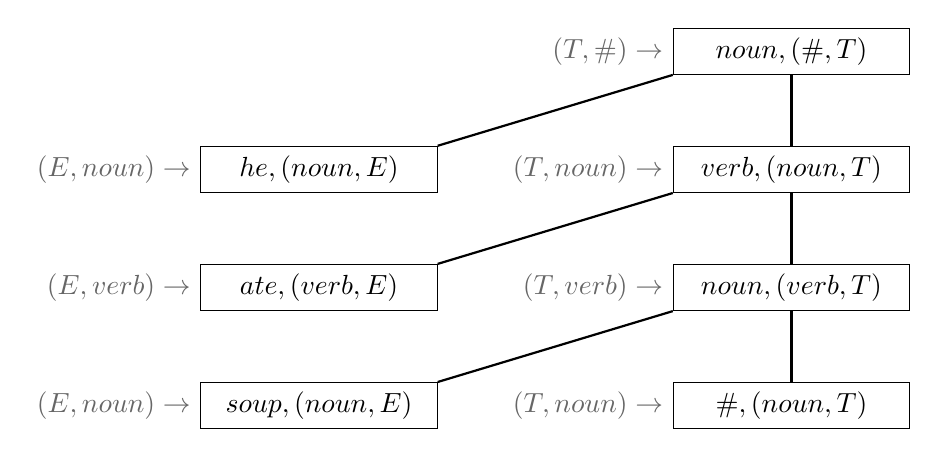
\begin{tikzpicture}[n/.style={rectangle,draw,minimum width=3cm},every label/.style={color={black!60}}]
  \node[n,label=left:{$(T,\#)\to$}](t0) at (0,0) { $\text{noun},(\#,T)$ };
  \node[n,label=left:{$(T,\text{noun})\to$}](t1) at (0,-1.5) { $\text{verb},(\text{noun},T)$ } edge[thick] (t0);
  \node[n,label=left:{$(T,\text{verb})\to$}](t2) at (0,-3.0) { $\text{noun},(\text{verb},T)$ } edge[thick] (t1);
  \node[n,label=left:{$(T,\text{noun})\to$}](t3) at (0,-4.5) { $\#,(\text{noun},T)$ }          edge[thick] (t2);
  \node[n,label=left:{$(E,\text{noun})\to$}](e1) at (-6,-1.5) { $\text{he},(\text{noun},E)$ };
  \node[n,label=left:{$(E,\text{verb})\to$}](e2) at (-6,-3.0) { $\text{ate},(\text{verb},E)$ };
  \node[n,label=left:{$(E,\text{noun})\to$}](e3) at (-6,-4.5) { $\text{soup},(\text{noun},E)$ };
  \draw[thick] (t0.south west) -- (e1.north east);
  \draw[thick] (t1.south west) -- (e2.north east);
  \draw[thick] (t2.south west) -- (e3.north east);
 \end{tikzpicture}
 \caption{
  Example for a hidden information $y\in Y_{\not\bot}\subseteq T_C$
  corresponding to the observation $x = \text{``He ate soup.''}$ and the state
  sequence ``noun-verb-noun''. The label to the left of each node shows which
  grammar state produces this particular subtree when $y$ is generated by $K$.
 \label{fig:03-example-y}}
\end{figure}

In order to describe hidden information $y\in Y_{\not\bot}$ as a ranked tree of countable
events from $C$, we assign a rank to each $c = \mbig\kla{a,(q,s)}\isin C$ as follows:
\begin{align*}
 \rk\mbig\kla{a,(q,s)} := \begin{cases}
  0 & \text{if } s = E, \\
  2 & \text{if } s = T \text{ and } a\neq\#, \\
  0 & \text{if } s = T \text{ and } a = \#.
 \end{cases}
\end{align*}

The intuition for this choice is that each transition event causes two further
events: the emission event in the state that was entered, and the transition
event into the state after that. Emission events do not result in further
events because of the Markov property, and a transition event into the $\#$
state marks the end of the stochastic process after which no further events
occur. This rank assignment results in trees such as the one in
Figure~\ref{fig:03-example-y}.

The trees $y\in Y_{\not\bot}$ are generated by the tree grammars $H(x)$ and $K$. We
define\footnote{The set of grammar states $Q_K$ is isomorphic to $B$, but the
components of each pair are swapped: We write $(s,q)\in Q_K$, but $(q,s)\in B$.
This deliberate choice provides a visual cue for distinguishing grammar states
from countable events.}
\label{eq:03-K}\[
 K := \mbig\brc{Q_K, (T,\#), R_K} \quad\text{where}\quad Q_K = \brc T \times Q_\# \cup \brc E \times Q
\]
and $R_K$ contains the following rules:
\label{eq:03-R_K}\begin{align*}
 (T,q) &\to \mbig\kla{q',(q,T)}\mbig\kla{(E,q'),(T,q')} &&\forall q\in Q_\# \text{ and } q'\in Q, \\
 (T,q) &\to \mbig\kla{\#,(q,T)} &&\forall q\in Q_\#, \\
 (E,q) &\to \mbig\kla{v,(q,E)} &&\forall q\in Q \text{ and } v\in V.
\end{align*}

The grammar $K$ is an RTG since each rule produces as much subtrees as the rank
of its label $(a,b)$. The IO information requires that $K$ have certain
properties: First, it must be unambiguous. Because each $c\in C$ is produced by
at most one rule from $R_K$, $K$ is deterministic and, hence, unambiguous
(see~page~\pageref{lemma:02-deterministic-is-unambiguous}). Furthermore, we
need to show the following lemma.

\begin{lemma}
 For every $\omega\in\Omega$, the PRTG $(K,p_\omega')$ is proper, where
 \[
  p'_\omega(\rho) := \begin{cases}
   q_\omega(a|b) & \text{if } \rho=\mbig\kla{q\to(a,b)(q_1,\ldots,q_k)}\isin R_K, \\
   0 & \text{if } \rho\notin R_K.
  \end{cases}
 \]
\end{lemma}

\begin{proof}
 The restriction of $p_\omega'$ to $R_K$, i.~e., that $p_\omega'(\rho)=0$ for all
 $\rho\notin R_K$, follows directly from the definition above. It remains to be seen
 that $p_\omega'\in\um(Q_K^*\times C|Q_K)$. For any $q\in Q_\#$, we have
 \begin{align*}
  &\hspace{1.5em} \sum_{q_1\cdots q_k,(a,b)} p_\omega'\underbrace{\mBig\kla{(q_1\cdots q_k,(a,b)\npipe(T,q)}}_{=\,(T,q)\to(a,b)(q_1,\ldots,q_k)} \\
  &= p_\omega'\mBig\kla{(T,q) \to \mbig\kla{\#,(q,T)}} + \sum_{q'\in Q} p_\omega'\mBig\kla{(T,q) \to \mbig\kla{q',(q,T)}\mbig\kla{(E,q'),(T,q')}} \\
  &= q_\omega\mbig\kla{\#,(q,T)} + \sum_{q'\in Q} q_\omega\mbig\kla{q',(q,T)} = t(\#|q) + \sum_{q'\in Q} t(q'|q) = \sum_{q'\in Q_\#} t(q'|q) = 1
 \end{align*}
 because $t\in\um(Q_\#|Q_\#)$. Analogously, for any $q\in Q$, it follows from $e\in\um(V|Q)$ that
 \begin{align*}
  \sum_{q_1\cdots q_k,(a,b)} p_\omega'\mbig\kla{(E,q)\to(a,b)(q_1,\ldots,q_k)}
  &= \sum_{v\in V} p_\omega'\mBig\kla{(E,q) \to \mbig\kla{v,(q,E)}} \\
  &= \sum_{v\in V} q_\omega\mbig\kla{v,(q,E)} = \sum_{v\in V} e(v|q) = 1.
  \qedhere
 \end{align*}
\end{proof}

Using $K$, we can define the set $Y$ of hidden information as
\[
 Y := \lang K \cup \brc\bot.
\]

\begin{figure}[t!]
 \begin{align*}
  \pi_X\left(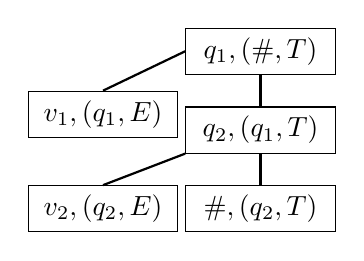
\begin{tikzpicture}[every node/.style={rectangle,draw,minimum width=1.9cm},baseline=(current bounding box.center)]
   \node (t0) at (0,0) { $q_1,(\#,T)$ };
   \node (t1) at (0,-1) { $q_2,(q_1,T)$ } edge[thick] (t0);
   \node (t2) at (0,-2) { $\#,(q_2,T)$ } edge[thick] (t1);
   \node (e1) at (-2,-0.8) { $v_1,(q_1,E)$ }; \draw [thick] (t0.west) -- (e1.north);
   \node (e2) at (-2,-2) { $v_2,(q_2,E)$ }; \draw [thick] (t1.south west) -- (e2.north);
  \end{tikzpicture}\right)
  &=
   \underbrace{\pi_X\bigl(v_1,(q_1,E)\bigr)}_{=v_1}
   \pi_X\left(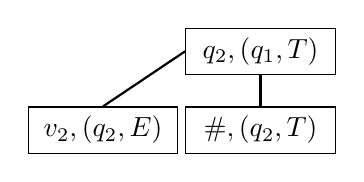
\begin{tikzpicture}[every node/.style={rectangle,draw,minimum width=1.9cm},baseline=(current bounding box.center)]
    \node (t1) at (0,0) { $q_2,(q_1,T)$ };
    \node (t2) at (0,-1) { $\#,(q_2,T)$ } edge[thick] (t1);
    \node (e2) at (-2,-1) { $v_2,(q_2,E)$ }; \draw [thick] (t1.west) -- (e2.north);
   \end{tikzpicture}\right)
  \\
  &= v_1
   \underbrace{\pi_X\bigl(v_2,(q_2,E)\bigr)}_{=v_2}
   \underbrace{\pi_X\bigl(\#,(q_2,T)\bigr)}_{=\eps}
   = v_1v_2
 \end{align*}
 \caption{\label{fig:03-readoff}%
  Example for how $\pi_X$ can be used to read the generated sentence from a tree $y\in Y_{\not\bot}$, where the HMM has states $Q = \{q_1,q_2,\ldots\}$ and words $V = \{v_1,v_2,\ldots\}$.
 }
\end{figure}

\label{def:03-def-pi-x}
Furthermore, we introduce a mapping $\pi_X: T_C \to V^*$ that reads the
generated sentence from a tree $t\in T_C$ (see Figure~\ref{fig:03-readoff}),
i.~e.,
\label{eq:03-pi_X}\[
 \pi_X(t) := \begin{cases}
  \eps & \text{if } t = \mbig\kla{\#,(q,T)} \text{ or } t = \mbig\kla{\#,(\#,E)}, \\
  v    & \text{if } t = \mbig\kla{v,(q,E)}, \\
  \pi_X(t_1)\pi_X(t_2) & \text{if } t = \mbig\kla{q',(q,T)}(t_1,t_2).
 \end{cases}
\]

From $\pi_X$, we derive the mapping $\pi_1: Y_{\not\bot} \to X_{\not\bot}$ that
the IO information requires by restricting the domain of $\pi_X$ to
$Y_{\not\bot}$\footnote{We cannot use the recursive definition of $\pi_X$ to
define $\pi_1$ directly, since the recursion goes over arguments from $T_C$
that are not all in $Y_{\not\bot}$.}, i.~e.,
\[
 \pi_1(y) := \pi_X(y) \quad\forall y\in Y_{\not\bot}.
\]

Finally, the IO information requires a mapping $H: X_{\not\bot}\to\ur(C)$ such
that $H(x)$ generates all $y$ with $\pi_1(y)=x$. We can define $H(x)$ by
starting from $K$, then restricting the set of rules such that only the
sentence $x$ can be generated.

\begin{definition}
 Let $x\in V^*$ be a sentence. We denote by $\suff(x)$ its
 \emph{set of suffixes}, including $x$ itself, but excluding the empty sentence, i.~e.,
 \[
  \suff(x) := \begin{cases}
   \emptyset & \text{if } x = \eps, \\
   \brc x \cup \suff(x') & \text{if } x = vx' \text{ with } v\in V\text{ and }x'\in V^*.
  \end{cases}\qedhere
 \]
\end{definition}

\begin{definition}
 The operators $\car\colon V^+\to V$ and $\cdr\colon V^+\to V^*$ decompose a nonempty sentence into its leading word and the rest of the sentence, i.~e., for any $x = v_1\cdots v_n\isin V^+$,
 \[
  \car(x) := v_1
  \quad\text{and}\quad
  \cdr(x) := v_2\cdots v_n.
  \qedhere
 \]
\end{definition}

For example, for $V = \brc{a,b,c}$ and $v = bbcb$, we have
\begin{align*}
 \suff(bbcb) &= \brc{bbcb, bcb, cb, b}, &
 \car(bbcb) &= b, &
 \cdr(bbcb) &= bcb.
\end{align*}
Using these operators, we define, for any $x\in X_{\not\bot} = V^*$,
\begin{align*}
 H(x) := \mbig\brc{Q_x,(T,\#,x),R_x} \quad\text{where}\quad
 Q_x &= \brc T \times Q_\# \times \mbig\kla{\suff(x)\cup\brc\eps} \\
 &\hspace{0.15em}\cup\hspace{0.15em} \brc E \times Q \times \suff(x)
\end{align*}
and $R_x$ contains the following rules:
\label{eq:03-R_x}\begin{align*}
 (T,q,x') &\to \mbig\kla{q',(q,T)}\mbig\kla{(E,q',x'),(T,q',\cdr(x'))} && \forall q\in Q_\#,q'\in Q,\text{ and }x'\in\suff(x), \\
 (T,q,\eps) &\to \mbig\kla{\#,(q,T)} && \forall q\in Q_\#, \\
 (E,q,x') &\to \mbig\kla{\car(x'),(q,E)} && \forall q\in Q\text{ and }x'\in\suff(x).
\end{align*}
%
A grammar state $q\in Q_x$ tracks both the state from $Q_\#$ that the HMM is
currently in, and the suffix of $x$ that has not yet been generated yet. Emission
rules are restricted such that only the leading word from that suffix can be generated.

For the empty sentence $x=\eps$, the initial grammar state $(T,\#,\eps)$ can
only be expanded using a rule of the second kind without producing any subsequent states.
We therefore have
\[
 \mbig\lang{H(\eps)} = \mBig\brc{\mbig\kla{\#,(\#,T)}}.
\]
%
Using the same reasoning as above for $K$, we see that each $H(x)$ is
deterministic and, therefore, unambiguous. It remains to be shown that
\[
 \forall x\in X_{\not\bot}\colon\;
 \mbig\lang{H(x)} = \pi_1^{-1}(x).
\]
We decompose the proof for this equivalence into two lemmas.

\begin{lemma}\label{lemma:03-consistent-yield}
 With the definitions shown above,
 \[
  \forall x\in X_{\not\bot}\colon\;
  \forall y\in \mbig\lang{H(x)}\colon\;
  \pi_1(y) = x.
 \]
\end{lemma}

\begin{lemma}\label{lemma:03-language-partition}
 With the definitions shown above,
 \[
  \mbig\lang K = \bigcup_{x\in X_{\not\bot}} \mbig\lang{H(x)}.
 \]
\end{lemma}

The proofs for these lemmas can be found in Appendix~\ref{sec:appendix-hk-proofs}. For each $x\in X_{\not\bot}$, we then have
\[
 \pi_1^{-1}(x)
 = \mbig\brc{y\in \underbrace{Y_{\not\bot}}_{=\lang K} \pipe \pi_1(y) = x}
 = \bigcup_{x'\in X_{\not\bot}} \mbig\brc{y\in\mbig\lang{H(x')} \pipe \pi_1(y) = x}
\]
by Lemma~\ref{lemma:03-language-partition}. Because of
Lemma~\ref{lemma:03-consistent-yield}, only $x'=x$ contributes
a nonempty set to this union, yielding
\[
 \pi_1^{-1}(x) = \mbig\brc{y\in\mbig\lang{H(x)} \pipe \pi_1(y) = x} = \mbig\lang{H(x)}
\]
as required by the definition of the IO information. By all the considerations
in this subsection, the tuple $\mu_\uh := (q,\pi_1,K,H)$ therefore fulfils
Definition~\ref{02:def-io-info} and is, in fact, an IO information.

\subsection{Inside weights}

Let $\omega = (t,e)\in\Omega$. The definition of the complete-data corpus
$c\!\dangle{\omega,\mu}$ is based on the family $\chi_{\omega,x}$ of
$C$-corpora, which in turn is defined in terms of the inside weights $\beta_x$
and outside weights $\alpha_x$ of the PRTG $\mbig\kla{H(x),p_\omega'}$ for all
$x\in X_{\not\bot}=V^*$. We therefore have to derive expressions for all these
components.

Let $x\in X_{\not\bot}=V^*$. Recall that inside weights can, in general, be
calculated by~\eqref{eq:02-beta} (see page~\pageref{eq:02-beta}).
Instantiation of this equation for $\mbig\kla{H(x),p_\omega'}$ yields
\[
 \beta_x(q) = \sum_{q\to(a,b)(q_1,\ldots,q_k)\isin R_x} q_\omega(a|b) \cdot \beta_x(q_1) \cdots \beta_x(q_k)
\]
for all $q\in Q_x$, which can be expanded to
\begin{align*}
 \beta_x(E,q,x') &= q_\omega\mbig\kla{\car(x')\npipe(q,E)} = e\mbig\kla{\car(x')\npipe q}
 && \forall q\in Q \text{ and } x'\in\suff(x), \\
 \beta_x(T,q,\eps) &= q_\omega\mbig\kla{\#\npipe(q,T)} = t(\#|q)
 && \forall q\in Q_\#, \\
 \beta_x(T,q,x') &= \sum_{q'\in Q} \underbrace{q_\omega\mbig\kla{q'\npipe(q,T)}}_{=t(q'|q)} \cdot \underbrace{\beta_x(E,q',x')}_{=e(\car(x')|q')} \cdot \beta_x\mbig\kla{T,q',\cdr(x')}
 && \forall q\in Q_\# \text{ and } x'\in\suff(x).
\end{align*}
States $(T,q,x')$ with $x'\neq\eps$ only exist for $x\neq\eps$. In this
case, let $x=x_1\cdots x_n\in V^+$. Then, each suffix $x'\in\suff(x)$ has the
form $x' = x_i\cdots x_n$ for some $i\in\brc{1,\ldots,n}$, and we have
\[
 \car(x') = x_i
 \quad\text{and}\quad
 \cdr(x') = x_{i+1} \cdots x_n,
\]
if we define $x_{n+1}\cdots x_n := \eps$ as a corner case. Putting all this into
the previous equation, we have
\[
 \beta_x(T,q,x_i\cdots x_n) = \sum_{q'\in Q} t(q'|q) \cdot e(x_i|q') \cdot \beta_x(T,q',x_{i+1}\cdots x_n).
\]
By comparing with~\eqref{eq:03-S_v} on page~\pageref{eq:03-S_v}, we see that, for $q\neq\#$ and $i>1$, the inside weights recover the backward weights, i.~e.,
\[
 \beta_x(T,q,x_i\cdots x_n) = S_x(i-1,q).
\]
Furthermore, for the initial grammar state $(T,\#,x)$, we have
\[
 \beta_x(T,\#,x) = \beta_x(T,\#,x_1\cdots x_n) = \sum_{q'\in Q} t(q'|q) \cdot e(x_1|q') \cdot \underbrace{\beta_x(T,q',x_2\cdots x_n)}_{=S_x(1,q)} = P(x)
\]
by~\eqref{eq:03-p-by-s}. The statement $\beta_x(T,\#,x) = P(x)$ also holds for $x=\eps$ because
\label{eq:03-beta-eps}\[
 \beta_\eps(T,\#,\eps) = t(\#|\#) = P(\eps).
\]

We technically also have nonzero inside weights for grammar states $(T,q,x)$
with $q\in Q$, and grammar states $(T,\#,x')$ with $x'\in\suff(x)\setminus\brc
x$. But those grammar states are not reachable, which is why their exact inside
weights bear no relevance for the remainder of this derivation.

\subsection{Outside weights}

As shown before, the outside weights form a linear equation system according
to~\eqref{eq:02-alpha} (see page~\pageref{eq:02-alpha}). Instantiation of this
equation for the PRTG $\mbig\kla{H(x),p_\omega'}$ yields
\[
 \alpha_x(q) = \delta_{(T,\#,x)}^q + \sum_{(q'\to(a,b)(q_1,\ldots,q_k))\in R_x, m:\,q_m=q} \alpha_x(q') \cdot q_\omega(a|b) \cdot \prod_{l\neq m} \beta_x(q_l)
\]
for all $q\in Q_x$. For all $x\in V^*$, we have
\label{eq:03-alpha-eps}\[
 \alpha_x(T,\#,x) = 1
\]
for the initial state, since it is not produced by any rule. For $x=\eps$, all
other outside weights vanish because no other grammar states can be produced.
Otherwise, let $x=x_1\cdots x_n\isin V^+$ so that, as before, every
$x'\in\suff(x)$ has the form $x'=x_i\cdots x_n$ for some
$i\in\brc{1,\ldots,n}$. Other than $\alpha_x(T,\#,x)$, we have nonzero
outside weights
\begin{align*}
 \alpha_x(T,q,x_{i+1}\cdots x_n) &= \sum_{q'\in Q_\#} \alpha_x(T,q',x_i\cdots x_n) \cdot \underbrace{q_\omega\mbig\kla{q\npipe(q',T)}}_{=t(q|q')} \cdot \underbrace{\beta_x(E,q,x_i\cdots x_n)}_{=e(x_i|q)} \\
 \text{and }
 \alpha_x(E,q,x_i\cdots x_n)     &= \sum_{q'\in Q_\#} \alpha_x(T,q',x_i\cdots x_n) \cdot \underbrace{q_\omega\mbig\kla{q\npipe(q',T)}}_{=t(q|q')} \cdot \underbrace{\beta_x(T,q,x_{i+1}\cdots x_n)}_{=S_x(i,q)},
\end{align*}
both for $i\in\brc{1,\ldots,n}$ and $q\in Q$. The grammar states $(T,q,x)$ with $q\neq\#$ are unreachable. For $i=1$, we therefore have
\[
 \alpha_x(T,q,x_2\cdots x_n) = \sum_{q'\in Q_\#} \underbrace{\alpha_x(T,q',x_1\cdots x_n)}_{\text{$1$ for $q'=\#$, $0$ otherwise}} \cdot\, t(q|q') \cdot e(x_1|q)
 = t(q|\#) \cdot e(x_1|q) = T_x(1,q).
\]
For $x'\neq x$, we can likewise observe that the grammar states $(T,\#,x')$ are
unreachable, hence the sum in $\alpha_x(T,q,x_{i+1}\cdots x_n)$ for $i>1$ goes
over $q'\in Q$ only. Comparison with~\eqref{eq:03-T_v} shows that
\[
 \alpha_x(T,q,x_{i+1}\cdots x_n) = T_x(i,q)
\]
for all $i\in\brc{1,\ldots,n}$ and $q\in Q$. Inserting these findings into the
outside weights of the states $(E,q,x_i\cdots x_n)$, we obtain, for $i=1$,
\begin{align*}
 \alpha_x(E,q,x_1\cdots x_n)
 &= \sum_{q'\in Q_\#} \underbrace{\alpha_x(T,q',x_1\cdots x_n)}_{\text{$1$ for $q'=\#$, $0$ otherwise}} \cdot\, t(q|q') \cdot S_x(1,q) \\
 &= t(q|\#) \cdot S_x(1,q)
 = \frac{T_x(1,q) \cdot S_x(1,q)}{e(x_1|q)},
\end{align*}
and for $i>1$, we likewise have
\begin{align*}
 \alpha_x(E,q,x_i\cdots x_n)
 &= \sum_{q'\in Q_\#} \underbrace{\alpha_x(T,q',x_i\cdots x_n)}_{0\text{ for }q'\,=\,\#} \cdot t(q|q') \cdot S_x(i,q) \\
 &= \sum_{q'\in Q} T_x(i-1,q') \cdot t(q|q') \cdot S_x(i,q)
 = \frac{T_x(i,q) \cdot S_x(i,q)}{e(x_i|q)}.
\end{align*}

\subsection{Complete-data corpus}

For the remainder of this chapter, let $c$ be a $V^*$-corpus, and
$\mu:=\mu_\uh$. The E-step of the IO step mapping involves the computation of
the complete-data corpus $c\!\dangle{\omega,\mu}$ according to
\[
 c\!\dangle{\omega,\mu}\!(a,b) = \sum_x c(x) \cdot \chi_{\omega,x}(a,b).
\]
We therefore need to derive expressions for all $\chi_{\omega,x}(a,b)$ first.
Following the definition of $\chi_{\omega,x}(a,b)$ in~\eqref{eq:02-chi} on
page~\pageref{eq:02-chi}, we have, in general,
\begin{equation}\label{eq:03-chi}
 \chi_{\omega,x}(a,b) = \underbrace{\beta_x(T,\#,x)^{-1}}_{=P(x)^{-1}} \cdot \sum_{(q\to(a,b)(q_1,\ldots,q_k))\in R_x} \alpha_x(q) \cdot q_\omega(a|b) \cdot \beta_x(q_1) \cdots \beta_x(q_k).
\end{equation}

For $x=\eps$, we only have one nonzero outside weight, $\alpha_\eps(T,\#,\eps)
= 1$, and only one rule that applies to this state, $(T,\#,\eps) \to
\mbig\kla{\#,(\#,T)}$, from which follows that
\[
 \chi_{\omega,\eps}\mbig\kla{\#,(\#,T)} = \underbrace{P(x)^{-1}}_{=t(\#|\#)^{-1}} \cdot \underbrace{\alpha_x(T,\#,\eps)}_{=1} \cdot \underbrace{q_\omega\mbig\kla{\#\npipe(\#,T)}}_{=t(\#|\#)} = 1
\]
and all other $\chi_{\omega,\eps}(a,b)$ vanish. Since $(T,\#,\eps)$ is
unreachable in all $H(x)$ with $x\neq\eps$, we have $\alpha_x(T,\#,\eps) = 0$
and therefore $\chi_{\omega,x}\mbig\kla{\#,(\#,T)}=0$ for all $x\neq\eps$, and finally,
\[
 c\!\dangle{\omega,\mu}\!\mbig\kla{\#,(\#,T)} = c(\eps) \cdot \underbrace{\chi_{\omega,\eps}\mbig\kla{\#,(\#,T)}}_{=1} + \sum_{x\neq\eps} c(x) \cdot \underbrace{\chi_{\omega,x}\mbig\kla{\#,(\#,T)}}_{=0} = c(\eps).
\]

This concludes the consideration of $x=\eps$. Let $x=x_1\cdots x_n\isin V^+$. For emission events
$\mbig\kla{v,(q,E)}$ with $v\in V$ and $q\in Q$, \eqref{eq:03-chi} leads to
\begin{align*}
 \chi_{\omega,x}\mbig\kla{v,(q,E)}
 &= P(x)^{-1} \cdot \sum_{i\in\brc{1,\ldots,n}:\, x_i=v} \underbrace{\alpha_x(E,q,x_i\cdots x_n)}_{=T_x(i,q)\cdot S_x(i,q)\cdot e(x_i|q)^{-1}} \cdot \underbrace{q_\omega\mbig\kla{v\npipe(q,E)}}_{=e(v|q)} \\
 &= \sum_{i\in\brc{1,\ldots,n}:\, x_i=v} \frac{T_x(i,q)\cdot S_x(i,q)}{P(x)}
  = \sum_{i\in\brc{1,\ldots,n}:\, x_i=v} R_x(i,q).
\end{align*}
For transition events into and out of the $\#$ state, we obtain, for any $q\in Q$,
\begin{align*}
 \chi_{\omega,x}\mbig\kla{\#,(q,T)}
 &= P(x)^{-1} \cdot \underbrace{\alpha_x(T,q,\eps)}_{=T_x(n,q)} \cdot \underbrace{q_\omega\mbig\kla{\#\npipe(q,T)}}_{=t(\#|q)=S_x(n,q)} = R_x(n,q), \\
 \text{and } \chi_{\omega,x}\mbig\kla{q,(\#,T)}
 &= P(x)^{-1} \cdot \sum_{x'\in\suff(x)} \underbrace{\alpha_x(T,\#,x')}_{=0\text{ for }x'\neq x} \cdot \underbrace{q_\omega\mbig\kla{q\npipe(\#,T)}}_{=t(q|\#)} \cdot \beta_x(E,q,x') \cdot \beta_x\mbig\kla{T,q,\cdr(x')} \\
 &= P(x)^{-1} \cdot \underbrace{\alpha_x(T,\#,x)}_{=1} \cdot t(q|\#) \cdot \underbrace{\beta_x(E,q,x)}_{=e(x_1|q)} \cdot \underbrace{\beta_x\mbig\kla{T,q,\cdr(x)}}_{=S_x(1,q)} \\
 &= P(x)^{-1} \cdot \underbrace{t(q|\#) \cdot e(x_1|q)}_{=T_x(1,q)} \cdot S_x(1,q)
  = R_x(1,q).
\end{align*}

For transition events from some $q\in Q$ to some $q'\in Q$, we initially get
\begin{align*}
 \chi_{\omega,x}\mbig\kla{q',(q,T)}
 &= P(x)^{-1} \cdot \sum_{x'\in\suff(x)} \alpha_x(T,q,x') \cdot \underbrace{q_\omega\mbig\kla{q'\npipe(q,T)}}_{=t(q'|q)} \cdot \beta_x(E,q',x') \cdot \beta_x\mbig\kla{T,q,\cdr(x')}. \\
 \intertext{To simplify this expression, we once more rewrite $\sum_{x'\in\suff(x)}$ into $\sum_{i=1}^n$ such that $x' = x_i\cdots x_n$.}
 \chi_{\omega,x}\mbig\kla{q',(q,T)}
 &= P(x)^{-1} \cdot \sum_{i=1}^n \,\underbrace{\alpha_x(T,q,x_i\cdots x_n)}_{=\,0\text{ for }i\,=\,1} \cdot t(q'|q) \cdot \underbrace{\beta_x(E,q',x_i\cdots x_n)}_{=e(x_i|q)} \cdot \underbrace{\beta_x\mbig\kla{T,q,x_{i+1}\cdots x_n}}_{=S_x(i,q)} \\
 &= P(x)^{-1} \cdot \sum_{i=2}^n \,\underbrace{\alpha_x(T,q,x_i\cdots x_n)}_{=T_x(i-1,q)} \cdot t(q'|q) \cdot e(x_i|q) \cdot S_x(i,q) \\
 &= \sum_{i=2}^n U_x(i-1,q,q') = \sum_{i=1}^{n-1} U_x(i,q,q').
\end{align*}

When we put these expressions into the definition of
$c\!\dangle{\omega,\mu}$, the sum over $x$ initially goes over all $x\in
V^+ = X_{\not\bot}\setminus\brc\eps$. However, we can restrict the sum to
$\operatorname{supp}(c)$ since the factor $c(x)$ makes every contribution from
outside $\operatorname{supp}(c)$ vanish. The sum therefore goes over
$\operatorname{supp}(c)\setminus\brc\eps$ only, which we shall denote by $X_c$.
For any $q,q'\in Q$ and $v\in V$, we finally have
\begin{align}\label{eq:03-c-dangle}
 c\!\dangle{\omega,\mu}\!\mbig\kla{\#,(\#,T)} &= c(\eps), \\
 c\!\dangle{\omega,\mu}\!\mbig\kla{\#,(q,T)} &= \sum_{x\in X_c} c(x) \cdot R_x\mbig\kla{\abs x\!,q}, &
 c\!\dangle{\omega,\mu}\!\mbig\kla{q',(q,T)} &= \sum_{x\in X_c} c(x) \cdot \sum_{i=1}^{\abs x-1} U_x(i,q,q'), \nonumber\\
 c\!\dangle{\omega,\mu}\!\mbig\kla{q,(\#,T)} &= \sum_{x\in X_c} c(x) \cdot R_x(1,q), &
 c\!\dangle{\omega,\mu}\!\mbig\kla{v,(q,E)} &= \sum_{x\in X_c} c(x) \cdot \sum_{{\scriptstyle i=1}\atop{\scriptstyle x_i=v}}^{\abs x} R_x(i,q). \nonumber
\end{align}

These equations are similar to~\eqref{eq:03-bw-start}
through~\eqref{eq:03-bw-end} aside from variable names and term ordering, with
one exception: Algorithm~\ref{alg:bw-vogler} operates on a $V^+$-corpus rather
than a $V^*$-corpus, so the empty sentence $\eps$ is not accounted for. Given
the $V^+$-corpus $h$, we can define the equivalent $V^*$-corpus $c_h$ by
\[
 c_h(x) := \begin{cases}
  h(x) &\text{if } x\in V^+, \\
  0 & \text{if } x=\eps.
 \end{cases}
\]
By using $c_h$ instead of $c$ in the equations~\eqref{eq:03-c-dangle}, and by noting that
\[
 \sum_{x\in X_{c_h}} = \sum_{x\in \operatorname{supp}(c_h)\setminus\brc\eps} = \sum_{x\in\operatorname{supp}(h)\setminus\brc\eps} = \sum_{x\in\operatorname{supp}(h)},
\]
we find that~\eqref{eq:03-bw-start} and~\eqref{eq:03-bw-end} are equivalent
to~\eqref{eq:03-c-dangle}. Therefore, after line~22 of
Algorithm~\ref{alg:bw-vogler},
\begin{equation}\label{eq:03-cnt-by-c}
 \cnt_\mathrm{tr}(q',q) = c_h\!\dangle{\omega,\mu}\!\mbig\kla{q',(q,T)}
 \quad\text{and}\quad
 \cnt_\mathrm{em}(v,q) = c_h\!\dangle{\omega,\mu}\!\mbig\kla{v,(q,E)}
\end{equation}
for all $(q',q)\in Q_\#\times Q_\#$ and $(v,q)\in V\times Q$, respectively. This equivalence
also shows how the Baum-Welch algorithm can be extended to allow for a
$V^*$-corpus instead of a $V^+$-corpus. The only difference is that
$\cnt_\mathrm{tr}(\#,\#)$ has to be set to $c(\eps)$ between lines~4 and~22.

\subsection{Step mapping}

Having calculated the complete-data corpus, we can apply the inside-outside
step mapping,
\[
 \stepmap\mu_\mathrm{io}(\omega) := \cmle_q\mbig\kla{c\mnorm\dangle{\omega,\mu}} = \argmax_{\omega'} q_{\omega'}\mbig\kla{c\mnorm\dangle{\omega,\mu}},
\]
then use it to choose a new model parameter $\hat\omega$ from this set.
According to Lemma~\ref{lemma:empirical3} (see
page~\pageref{lemma:empirical3}), we can choose $\hat\omega$ such that
$q_{\hat\omega} = \widetilde{c\!\dangle{\omega,\mu}}$ if such a
$\hat\omega$ exists.

\begin{lemma}
 For any $p\in\um_C(A|B)$, there exists $\omega=(t,e)\in\Omega$ such that $q_\omega = p$.
\end{lemma}

\begin{proof}
 The $\omega=(t,e)$ in question is given by
 \begin{align*}
  t(q'|q) &:= p\mbig\kla{q'\npipe(q,T)} &&\forall q,q'\in Q_\#, \\
  e(v|q) &:= p\mbig\kla{v\npipe(q,E)} &&\forall v\in V,q\in Q.
 \end{align*}
 We need to show that $\omega\in\Omega$ and $q_\omega=p$. Since $p\in\um(A|B)$,
 it holds for any $q\in Q_\#$ that
 \[
  \sum_{q'\in Q_\#} t(q'|q) = \sum_{q'\in Q_\#} p\mbig\kla{q'\npipe(q,T)} = 1.
 \]
 Therefore, $t\in\um(Q_\#|Q_\#)$. By an analogous argument, we have
 $e\in\um(V|Q)$, from which follows $\omega\in\Omega$. Moreover, for any
 $(a,b)\in A\times B$, we have
 \[
  q_\omega(a|b) = \begin{cases}
   p(a|b) & \text{if } (a,b)\in C, \\
   0 & \text{otherwise}
  \end{cases}
 \]
 because of how $q$ is defined. This is equivalent to saying that $q_\omega=p$
 since $p\in\um_C(A|B)$ is restricted to $C$.
\end{proof}

Since $c\!\dangle{\omega,\mu}$ is restricted to $C$ (i.~e., zero-valued
anywhere outside $C$), we have
$\widetilde{c\!\dangle{\omega,\mu}}\in\um_C(A|B)$. We can therefore apply the
construction for $t$ and $e$ from this proof to obtain $\hat\omega=(\hat t,\hat
e)$ which is in $\stepmap\mu_\mathrm{io}(\omega)$.
\begin{align*}
 \hat t(q'|q) &:= \widetilde{c\!\dangle{\omega,\mu}}\mbig\kla{q'\npipe(q,T)} &&\forall q,q'\in Q_\#, \\
 \hat e(v|q) &:= \widetilde{c\!\dangle{\omega,\mu}}\mbig\kla{v\npipe(q,E)} &&\forall v\in V,q\in Q.
\end{align*}

In the case of Algorithm~\ref{alg:bw-vogler}, we have $c=c_h$, and the
equations~\eqref{eq:03-cnt-by-c} apply. We therefore have, for every $q,q'\in
Q_\#$ and $v\in V$,
\begin{align*}
 \hat t(q'|q)
 &= \widetilde{c\!\dangle{\omega,\mu}}\mbig\kla{q'\npipe(q,T)}
 = \frac{c\!\dangle{\omega,\mu}\!\mbig\kla{q'\npipe(q,T)}}{\sum_{q''\in Q_\#}c\!\dangle{\omega,\mu}\!\mbig\kla{q''\npipe(q,T)}}
 \overset{\eqref{eq:03-cnt-by-c}}= \frac{\cnt_\mathrm{tr}(q',q)}{\sum_{q''\in Q_\#} \cnt_\mathrm{tr}(q'',q)}, \\
 \hat e(v|q)
 &= \widetilde{c\!\dangle{\omega,\mu}}\mbig\kla{v\npipe(q,E)}
 = \frac{c\!\dangle{\omega,\mu}\!\mbig\kla{v\npipe(q,E)}}{\sum_{v'\in V}c\!\dangle{\omega,\mu}\!\mbig\kla{v'\npipe(q,E)}}
 \overset{\eqref{eq:03-cnt-by-c}}= \frac{\cnt_\mathrm{em}(v,q)}{\sum_{v'\in V} \cnt_\mathrm{em}(v',q)}.
\end{align*}

Comparison with Algorithm~\ref{alg:bw-vogler} shows that this is exactly the
same computation carried out by lines 23--28. In total, we see that each
iteration of the main loop of this algorithm takes in a previous $\omega=(t,e)$
and computes $\hat\omega=(\hat t,\hat e)$ such that $\hat\omega\in\stepmap\mu_\mathrm{io}(\omega)$.
This is the same behavior that we described more abstractly in
Algorithm~\ref{alg:skeleton} (see page~\pageref{alg:skeleton}). This shows that
the Baum-Welch algorithm is, in fact, an instance of the EM algorithm from
\cite{bucstuvog15} that was introduced in Chapter~2, and consequently, that the
convergence properties of the generic EM algorithm apply to it as well.
